\documentclass[11pt,a4paper]{article}

\usepackage[margin=22mm]{geometry}
\usepackage[T1]{fontenc}
\usepackage[utf8]{inputenc}
\usepackage{lmodern}
\usepackage{xcolor}
\usepackage{booktabs}
\usepackage{tabularx}
\usepackage{array}
\usepackage{amsmath}
\usepackage{xspace}
\usepackage{enumitem}
\usepackage{listings}
\usepackage{tikz}
\usetikzlibrary{arrows.meta,positioning,fit,shapes.geometric,calc,backgrounds}
\usepackage[colorlinks=true,linkcolor=blue!55!black,urlcolor=blue!55!black]{hyperref}

\definecolor{LyraBlue}{HTML}{315C8C}
\definecolor{LyraGreen}{HTML}{2F7D5B}
\definecolor{LyraAmber}{HTML}{B46B17}
\definecolor{LyraRed}{HTML}{A53A3A}
\definecolor{LyraGray}{HTML}{5C6670}
\definecolor{CodeBg}{HTML}{F4F6F8}

\lstdefinestyle{lyraform}{
  basicstyle=\ttfamily\small,
  backgroundcolor=\color{CodeBg},
  frame=single,
  rulecolor=\color{black!18},
  columns=fullflexible,
  keepspaces=true,
  showstringspaces=false,
  breaklines=true,
  xleftmargin=4pt,
  xrightmargin=4pt
}

\tikzset{
  operation/.style={draw=LyraBlue, very thick, rounded corners, fill=LyraBlue!7,
    align=center, minimum width=31mm, minimum height=10mm},
  consumer/.style={draw=LyraAmber, very thick, rounded corners, fill=LyraAmber!9,
    align=center, minimum width=31mm, minimum height=10mm},
  success/.style={draw=LyraGreen, thick, rounded corners, fill=LyraGreen!9,
    align=center, minimum width=28mm, minimum height=9mm},
  failure/.style={draw=LyraRed, thick, rounded corners, fill=LyraRed!8,
    align=center, minimum width=30mm, minimum height=9mm},
  fault/.style={draw=black!65, thick, rounded corners, fill=black!7,
    align=center, minimum width=27mm, minimum height=9mm},
  policy/.style={draw=LyraGray, thick, dashed, rounded corners, fill=LyraGray!7,
    align=center, minimum width=29mm, minimum height=9mm},
  refused/.style={draw=LyraRed, very thick, rounded corners, fill=LyraRed!15,
    align=center, minimum width=30mm, minimum height=10mm},
  wire/.style={-{Latex[length=2.6mm]}, thick},
  successwire/.style={wire, draw=LyraGreen},
  failurewire/.style={wire, draw=LyraRed},
  faultwire/.style={wire, draw=black!70},
  policywire/.style={wire, draw=LyraGray, dashed},
  labelbox/.style={fill=white, inner sep=1.5pt, font=\scriptsize}
}

\newcommand{\canonical}{\textcolor{LyraGreen}{\textbf{Canonical}}\xspace}
\newcommand{\provisional}{\textcolor{LyraAmber}{\textbf{Provisional projection}}\xspace}
\newcommand{\notadmitted}{\textcolor{LyraRed}{\textbf{Not admitted}}\xspace}
\newcommand{\code}[1]{\texttt{#1}}

\title{Lyraform Failure Flow\\Semantic--Syntax--Graph Projection Map}
\author{Lyraform architecture note}
\date{2026-10-07}

\begin{document}
\maketitle

\begin{center}
\fcolorbox{LyraAmber}{LyraAmber!8}{\parbox{0.91\linewidth}{
\textbf{Document status: design map, not a syntax decision.}
The semantic laws and shared contracts cited here are authoritative. Surface
syntax and general executable graph behavior remain provisional until accepted
and implemented by later bounded stages. Examples marked ``provisional'' must
not be treated as currently accepted Lyraform programs.
}}
\end{center}

\section{One authority, three projections}

Lyraform uses one canonical semantic authority and permits multiple faithful
projections. Source syntax declares intent. Canonical semantic facts establish
identity, type, legality, obligation, commit law, and provenance. A graph then
projects those already-decided facts as typed ports and wires.

\begin{center}
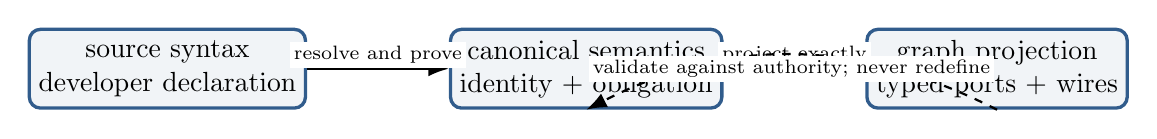
\begin{tikzpicture}[node distance=18mm]
  \node[operation] (syntax) {source syntax\\developer declaration};
  \node[operation, right=of syntax] (semantic) {canonical semantics\\identity + obligation};
  \node[operation, right=of semantic] (graph) {graph projection\\typed ports + wires};
  \draw[wire] (syntax) -- node[labelbox, above]{resolve and prove} (semantic);
  \draw[wire] (semantic) -- node[labelbox, above]{project exactly} (graph);
  \draw[wire, dashed, bend right=27] (graph.south) to
    node[labelbox, below]{validate against authority; never redefine} (semantic.south);
\end{tikzpicture}
\end{center}

The controlling rule is:

\begin{center}
\fbox{\parbox{0.88\linewidth}{
Syntax and graphs may expose semantics. They may not invent, weaken, infer away,
or silently terminate semantics. A backend executes an admitted graph; it does
not decide whether the graph was legal.
}}
\end{center}

\section{Disposition algebra and maturity}

Construction or semantic \emph{refusal} occurs before execution and creates no
runtime attempt. Every admitted runtime attempt completes exactly once as:

\[
  \operatorname{Attempt}(T,E,F)
  \longrightarrow
  \operatorname{Success}\langle T\rangle
  \;\mid\;
  \operatorname{Failure}\langle E\rangle
  \;\mid\;
  \operatorname{Fault}\langle F\rangle .
\]

\begin{center}
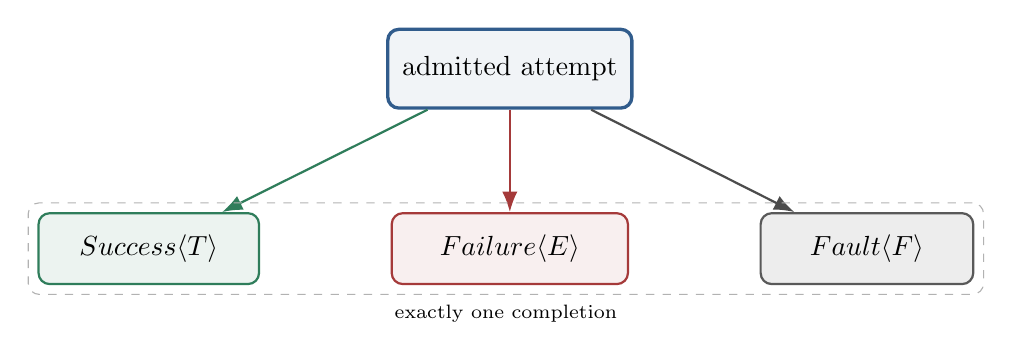
\begin{tikzpicture}[node distance=13mm and 16mm]
  \node[operation] (attempt) {admitted attempt};
  \node[success, below left=of attempt] (ok) {$Success\langle T\rangle$};
  \node[failure, below=of attempt] (fail) {$Failure\langle E\rangle$};
  \node[fault, below right=of attempt] (fault) {$Fault\langle F\rangle$};
  \draw[successwire] (attempt) -- (ok);
  \draw[failurewire] (attempt) -- (fail);
  \draw[faultwire] (attempt) -- (fault);
  \node[draw=black!30, dashed, rounded corners, fit=(ok)(fail)(fault),
    label=below:{\scriptsize exactly one completion}] {};
\end{tikzpicture}
\end{center}

\small
\begin{tabularx}{0.96\linewidth}{>{\bfseries\raggedright\arraybackslash}p{29mm}
  >{\raggedright\arraybackslash}X
  >{\raggedright\arraybackslash}p{34mm}}
\toprule
Concept & Current authority & Maturity \\
\midrule
Exclusive completion & Three exclusive typed dispositions & \canonical \\
No dangling unsuccessful route & Every failure/fault needs one accountable semantic destination & \canonical \\
Typed failure consumer & Closed accepted set and exact ordinary response-function identities & \canonical \\
Policy selection & Selects only a route already authorized by semantics & \canonical \\
Response transition & Bounded \code{recover} and \code{transform} contracts & \canonical, declarative \\
Surface spelling & Consumer, route, envelope, and transition declarations & \provisional \\
General graph execution & Failure ports, routing, response invocation, and rejoin & \notadmitted \\
Propagation, retry, sinks & Require separate contracts and bounded policy & \notadmitted \\
\bottomrule
\end{tabularx}
\normalsize

\section{How to read each operation map}

Each map uses the following sequence:

\begin{enumerate}[leftmargin=*,nosep]
  \item \textbf{Syntax projection}: a concise discussion notation. It is not
        accepted source syntax unless explicitly marked canonical.
  \item \textbf{Semantic interpretation}: the exact facts that must exist.
  \item \textbf{Graph projection}: ports and wires that preserve those facts.
  \item \textbf{Admission boundary}: what remains refused today.
\end{enumerate}

The provisional notation deliberately resembles Lyraform without selecting a
final keyword family. Square-bracket declarations such as
\code{[fails E]} and \code{[respond ...]} mean ``a future source projection
must express this fact''; the brackets are explanatory notation, not proposed
tokens.

\section{Operation 0: compile-time refusal}

\subsection*{Syntax projection}

Existing guard-oriented source can be statically contradictory:

\begin{lstlisting}[style=lyraform]
x : int(1)
positive : guard x > 0
-1 -> x
\end{lstlisting}

\subsection*{Semantic interpretation}

The compiler proves the predicate false before execution. The placement is
refused. There is no runtime attempt, no \code{Failure<GuardViolation>}, and no
graph node for the invalid placement.

\subsection*{Graph projection}

\begin{center}
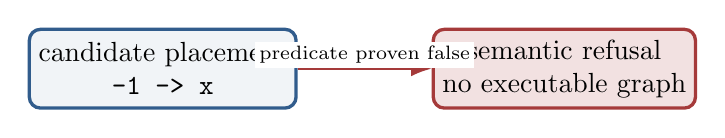
\begin{tikzpicture}[node distance=17mm]
  \node[operation] (source) {candidate placement\\\code{-1 -> x}};
  \node[refused, right=of source] (refusal) {semantic refusal\\no executable graph};
  \draw[wire, draw=LyraRed] (source) -- node[labelbox, above]{predicate proven false} (refusal);
\end{tikzpicture}
\end{center}

\textbf{Status:} \canonical. Refusal must not be reinterpreted as a runtime
failure merely to make the source executable.

\section{Operation 1: fallible runtime attempt}

\subsection*{Syntax projection}

\begin{lstlisting}[style=lyraform]
reading : int(1)
positive : guard reading > 0
read_sensor() -> reading

[read_sensor may complete as Failure<ReadFailure>]
[guard overwatch may complete as Failure<GuardViolation>]
\end{lstlisting}

The ordinary call and placement forms exist. The bracketed failure declarations
are provisional because general function failure effects and runtime guard
routing do not yet have admitted source spelling.

\subsection*{Semantic interpretation}

The operation has one stable identity and a closed set of possible exclusive
dispositions. A successful guarded commit produces
\code{Success<CommittedTransition>}; a rejected runtime candidate produces
\code{Failure<GuardViolation>} with no guarded-state commit. Contradictory
trusted evidence produces a separate fault.

\subsection*{Graph projection}

\begin{center}
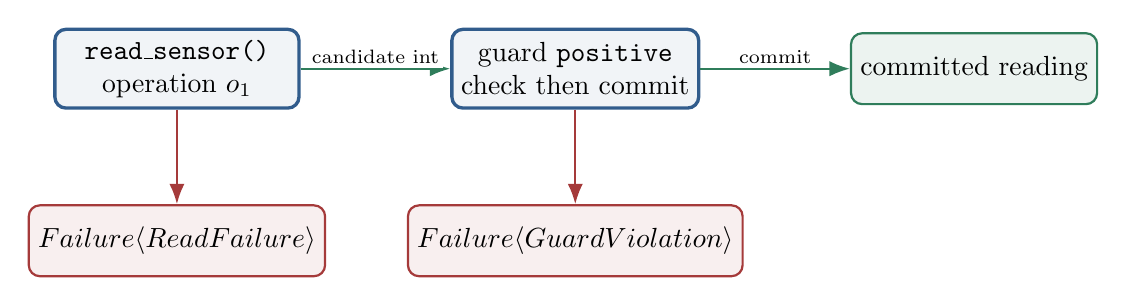
\begin{tikzpicture}[node distance=12mm and 19mm]
  \node[operation] (read) {\code{read\_sensor()}\\operation $o_1$};
  \node[operation, right=of read] (guard) {guard \code{positive}\\check then commit};
  \node[success, right=of guard] (commit) {committed reading};
  \node[failure, below=of read] (readfail) {$Failure\langle ReadFailure\rangle$};
  \node[failure, below=of guard] (guardfail) {$Failure\langle GuardViolation\rangle$};
  \draw[successwire] (read) -- node[labelbox, above]{candidate int} (guard);
  \draw[successwire] (guard) -- node[labelbox, above]{commit} (commit);
  \draw[failurewire] (read) -- (readfail);
  \draw[failurewire] (guard) -- (guardfail);
\end{tikzpicture}
\end{center}

\textbf{Status:} disposition meaning is \canonical; the shown runtime guard
and graph execution are \notadmitted until producer association and routing exist.

\section{Operation 2: declare a typed failure consumer}

\subsection*{Syntax projection}

\begin{lstlisting}[style=lyraform]
[consumer sensor_failures accepts {
    ReadFailure       => poll_sensor,
    GuardViolation    => use_safe_reading
}]

fn poll_sensor(failure : [FailureEnvelope<ReadFailure>]) : int {
    ...
}

fn use_safe_reading(failure : [FailureEnvelope<GuardViolation>]) : int {
    ...
}
\end{lstlisting}

Function declarations are existing language structure. The consumer block and
envelope type spelling are provisional projections of an already-canonical
contract; generic carrier syntax is not admitted here.

\subsection*{Semantic interpretation}

The \code{lyraform.failure\_consumer/v1} fact establishes:

\begin{itemize}[leftmargin=*,nosep]
  \item one consumer and declaration-scope identity;
  \item a closed accepted failure payload-type set;
  \item exact route identities;
  \item exact ordinary function-symbol identity for every route;
  \item exact typed \code{failure\_envelope} input projection;
  \item definition availability and a non-void result.
\end{itemize}

Names such as \code{poll\_sensor} remain developer names. The compiler routes by
resolved identity and type, never by matching a name string.

\subsection*{Graph projection}

\begin{center}
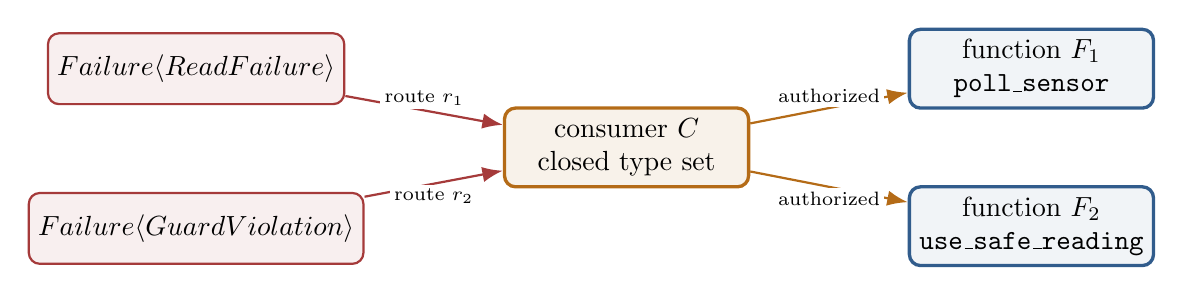
\begin{tikzpicture}[node distance=11mm and 20mm]
  \node[failure] (readfail) {$Failure\langle ReadFailure\rangle$};
  \node[failure, below=of readfail] (guardfail) {$Failure\langle GuardViolation\rangle$};
  \node[consumer, right=of readfail, yshift=-10mm] (consumer) {consumer $C$\\closed type set};
  \node[operation, right=of consumer, yshift=10mm] (poll) {function $F_1$\\\code{poll\_sensor}};
  \node[operation, right=of consumer, yshift=-10mm] (safe) {function $F_2$\\\code{use\_safe\_reading}};
  \draw[failurewire] (readfail) -- node[labelbox, above]{route $r_1$} (consumer);
  \draw[failurewire] (guardfail) -- node[labelbox, below]{route $r_2$} (consumer);
  \draw[wire, draw=LyraAmber] (consumer) -- node[labelbox, above]{authorized} (poll);
  \draw[wire, draw=LyraAmber] (consumer) -- node[labelbox, below]{authorized} (safe);
\end{tikzpicture}
\end{center}

\textbf{Status:} consumer semantics are \canonical and declarative. Syntax and
function invocation remain \provisional.

\section{Operation 3: policy selects an authorized route}

\subsection*{Syntax or policy projection}

Policy is not automatically language source. A discussion projection is:

\begin{lstlisting}[style=lyraform]
[policy field_profile revision "7" {
    sensor_failures.ReadFailure => route poll_sensor
}]
\end{lstlisting}

\subsection*{Semantic interpretation}

\code{lyraform.failure\_policy\_selection/v1} binds the policy identity and
revision to an exact consumer, failure type, and already-authorized route.
Policy cannot add a function, change a type, erase an obligation, or manufacture
success.

\subsection*{Graph projection}

\begin{center}
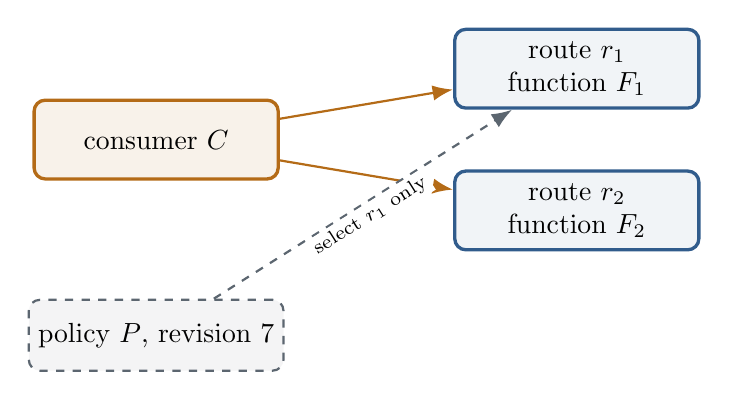
\begin{tikzpicture}[node distance=15mm and 22mm]
  \node[consumer] (consumer) {consumer $C$};
  \node[operation, right=of consumer, yshift=9mm] (f1) {route $r_1$\\function $F_1$};
  \node[operation, right=of consumer, yshift=-9mm] (f2) {route $r_2$\\function $F_2$};
  \node[policy, below=of consumer] (policy) {policy $P$, revision $7$};
  \draw[wire, draw=LyraAmber] (consumer) -- (f1);
  \draw[wire, draw=LyraAmber] (consumer) -- (f2);
  \draw[policywire] (policy) -- node[labelbox, below, sloped]{select $r_1$ only} (f1);
\end{tikzpicture}
\end{center}

\textbf{Status:} selection semantics are \canonical and declarative. Concrete
policy syntax, loading, and runtime activation remain \provisional.

\section{Operation 4: recover a failure into normal flow}

\subsection*{Syntax projection}

\begin{lstlisting}[style=lyraform]
fn use_safe_reading(
    failure : [FailureEnvelope<GuardViolation>]
) : int {
    1 -> return
}

[respond sensor_failures.GuardViolation
    with use_safe_reading
    as recover int]
\end{lstlisting}

The function remains ordinary. The provisional response declaration gives its
successful completion a semantic meaning; the function name does not.

\subsection*{Semantic interpretation}

The response-transition fact binds one exact consumer, route, function, and
incoming failure type. For \code{recover} it requires:

\[
  Failure\langle E\rangle
  \xrightarrow[\text{function }F]{\text{declared recover}}
  Success\langle T\rangle .
\]

The ordinary function result type must equal $T$. Successful response closes
the original expected-failure obligation, preserves the originating commit
evidence, and links response provenance to the origin. It does not rewrite the
failed attempt into a historical success.

\subsection*{Graph projection}

\begin{center}
\resizebox{\linewidth}{!}{%
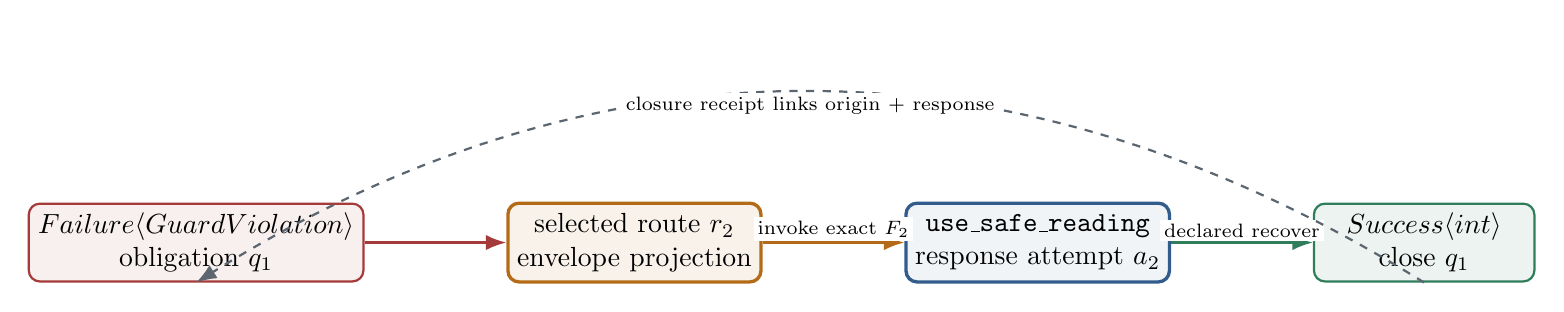
\begin{tikzpicture}[node distance=14mm and 18mm]
  \node[failure] (incoming) {$Failure\langle GuardViolation\rangle$\\obligation $q_1$};
  \node[consumer, right=of incoming] (consumer) {selected route $r_2$\\envelope projection};
  \node[operation, right=of consumer] (function) {\code{use\_safe\_reading}\\response attempt $a_2$};
  \node[success, right=of function] (success) {$Success\langle int\rangle$\\close $q_1$};
  \draw[failurewire] (incoming) -- (consumer);
  \draw[wire, draw=LyraAmber] (consumer) -- node[labelbox, above]{invoke exact $F_2$} (function);
  \draw[successwire] (function) -- node[labelbox, above]{declared recover} (success);
  \draw[wire, dashed, bend right=32, draw=LyraGray] (success.south) to
    node[labelbox, below]{closure receipt links origin + response} (incoming.south);
\end{tikzpicture}
}
\end{center}

\textbf{Status:} the response-transition semantics are \canonical and
declarative. Source spelling, invocation, rejoin rules, and execution remain
\notadmitted.

\section{Operation 5: transform one failure into another}

\subsection*{Syntax projection}

\begin{lstlisting}[style=lyraform]
fn classify_network_failure(
    failure : [FailureEnvelope<ResourceUnavailable>]
) : NetworkUnavailable {
    ... -> return
}

[respond network_failures.ResourceUnavailable
    with classify_network_failure
    as transform NetworkUnavailable]
\end{lstlisting}

\subsection*{Semantic interpretation}

For \code{transform}, successful completion produces a new typed failure:

\[
  Failure\langle E\rangle[q_1]
  \xrightarrow[\text{function }F]{\text{declared transform}}
  Failure\langle E_2\rangle[q_2],
  \qquad parent(q_2)=q_1 .
\]

The function result type must equal $E_2$. The original obligation is not
dropped: it is replaced by a linked successor obligation. Origin commit facts
remain immutable, and provenance records both the original producer and the
transforming response.

\subsection*{Graph projection}

\begin{center}
\resizebox{\linewidth}{!}{%
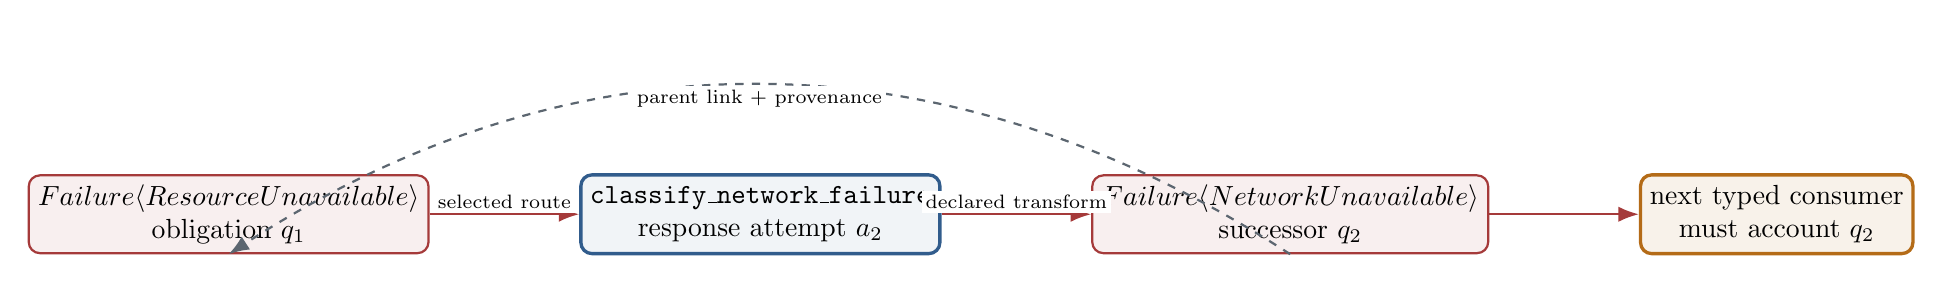
\begin{tikzpicture}[node distance=15mm and 19mm]
  \node[failure] (incoming) {$Failure\langle ResourceUnavailable\rangle$\\obligation $q_1$};
  \node[operation, right=of incoming] (function) {\code{classify\_network\_failure}\\response attempt $a_2$};
  \node[failure, right=of function] (outgoing) {$Failure\langle NetworkUnavailable\rangle$\\successor $q_2$};
  \node[consumer, right=of outgoing] (next) {next typed consumer\\must account $q_2$};
  \draw[failurewire] (incoming) -- node[labelbox, above]{selected route} (function);
  \draw[failurewire] (function) -- node[labelbox, above]{declared transform} (outgoing);
  \draw[failurewire] (outgoing) -- (next);
  \draw[wire, dashed, bend right=33, draw=LyraGray] (outgoing.south) to
    node[labelbox, below]{parent link + provenance} (incoming.south);
\end{tikzpicture}
}
\end{center}

\textbf{Status:} transform semantics are \canonical and declarative. The graph
must remain non-executable until successor routing is complete.

\section{Operation 6: the response attempt itself fails or faults}

\subsection*{Syntax projection}

\begin{lstlisting}[style=lyraform]
[respond ResourceUnavailable with poll_sensor as recover int]

[poll_sensor itself may complete as
    Failure<PollUnavailable> | Fault<ProviderIntegrityFault>]
\end{lstlisting}

\subsection*{Semantic interpretation}

The declared recover/transform class describes only \emph{successful completion}
of the response function. If the response attempt fails, it creates another
explicit obligation. If it faults, containment policy owns that evidence.
Neither event silently discharges the original failure.

\subsection*{Graph projection}

\begin{center}
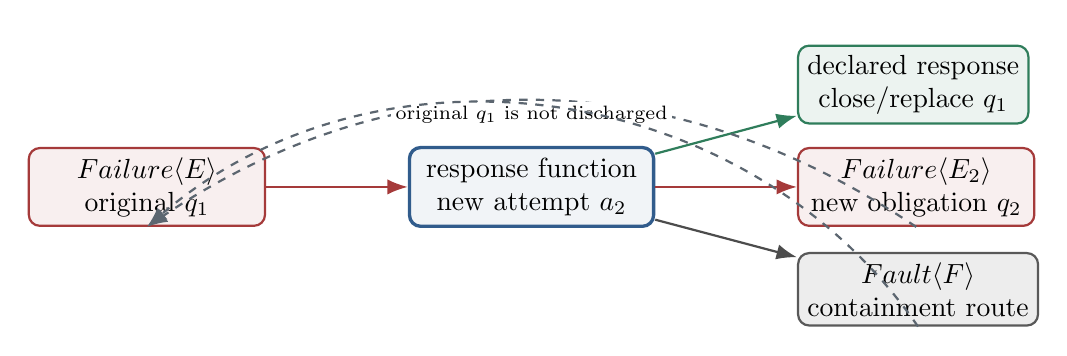
\begin{tikzpicture}[node distance=13mm and 18mm]
  \node[failure] (incoming) {$Failure\langle E\rangle$\\original $q_1$};
  \node[operation, right=of incoming] (response) {response function\\new attempt $a_2$};
  \node[success, right=of response, yshift=13mm] (ok) {declared response\\close/replace $q_1$};
  \node[failure, right=of response] (fail) {$Failure\langle E_2\rangle$\\new obligation $q_2$};
  \node[fault, right=of response, yshift=-13mm] (fault) {$Fault\langle F\rangle$\\containment route};
  \draw[failurewire] (incoming) -- (response);
  \draw[successwire] (response) -- (ok);
  \draw[failurewire] (response) -- (fail);
  \draw[faultwire] (response) -- (fault);
  \draw[wire, dashed, bend right=34, draw=LyraGray] (fail.south) to
    node[labelbox, below]{original $q_1$ is not discharged} (incoming.south);
  \draw[wire, dashed, bend right=48, draw=LyraGray] (fault.south) to (incoming.south);
\end{tikzpicture}
\end{center}

\textbf{Status:} the separate-obligation law is \canonical. General function
failure/fault declarations and executable routing are \notadmitted.

\section{Operation 7: dangling-wire refusal}

\subsection*{Syntax projection}

\begin{lstlisting}[style=lyraform]
read_sensor() -> reading

// ReadFailure is possible, but no consumer, propagation,
// policy sink, or containment route accounts for it.
\end{lstlisting}

\subsection*{Semantic interpretation}

An unsuccessful disposition is never optional. Logging and diagnostics may
observe it but do not consume it. Missing, ambiguous, or incomplete routing is
a compile-time dangling-wire refusal.

\subsection*{Graph projection}

\begin{center}
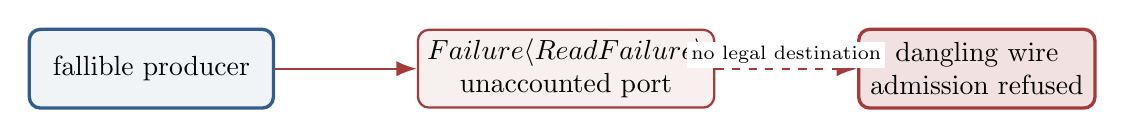
\begin{tikzpicture}[node distance=18mm]
  \node[operation] (producer) {fallible producer};
  \node[failure, right=of producer] (port) {$Failure\langle ReadFailure\rangle$\\unaccounted port};
  \node[refused, right=of port] (refusal) {dangling wire\\admission refused};
  \draw[failurewire] (producer) -- (port);
  \draw[wire, draw=LyraRed, dashed] (port) -- node[labelbox, above]{no legal destination} (refusal);
\end{tikzpicture}
\end{center}

\textbf{Status:} \canonical. A backend, logger, debugger, or default runtime
termination rule may not repair this graph.

\section{Identity-preserving projection table}

\small
\begin{tabularx}{\linewidth}{>{\bfseries\raggedright\arraybackslash}p{31mm}
  >{\raggedright\arraybackslash}X
  >{\raggedright\arraybackslash}X}
\toprule
Canonical fact & Possible source projection & Required graph projection \\
\midrule
Operation identity & Existing call, placement, guard, provider, or declaration origin & Stable producer-node identity \\
Exclusive dispositions & Future declared result/failure/fault contract & Distinct typed success, failure, and fault ports \\
Consumer identity & Future consumer declaration or scope projection & Consumer node/region with a closed accepted type set \\
Route identity & Future route declaration resolved to a function symbol & One typed wire to one exact response-function node \\
Policy selection & External policy artifact or future policy declaration & Selection edge annotates an existing route; creates none \\
Failure envelope & Future read-only parameter projection & Wire payload references producer, attempt, obligation, commit, and provenance \\
Recover transition & Future response annotation bound to an ordinary function & Success edge closes the incoming obligation \\
Transform transition & Future response annotation bound to an ordinary function & Failure edge creates a linked successor obligation \\
Response-attempt failure & Future function disposition declaration & Separate failure port and new must-account obligation \\
Fault & Future fault contract/containment association & Distinct containment wire; never ordinary recovery by default \\
\bottomrule
\end{tabularx}
\normalsize

\section{Complete bounded recover flow}

The following is the first intended end-to-end shape. Only the central semantic
contracts are currently implemented; source and executable graph projections
remain deliberately open.

\begin{center}
\resizebox{\textwidth}{!}{%
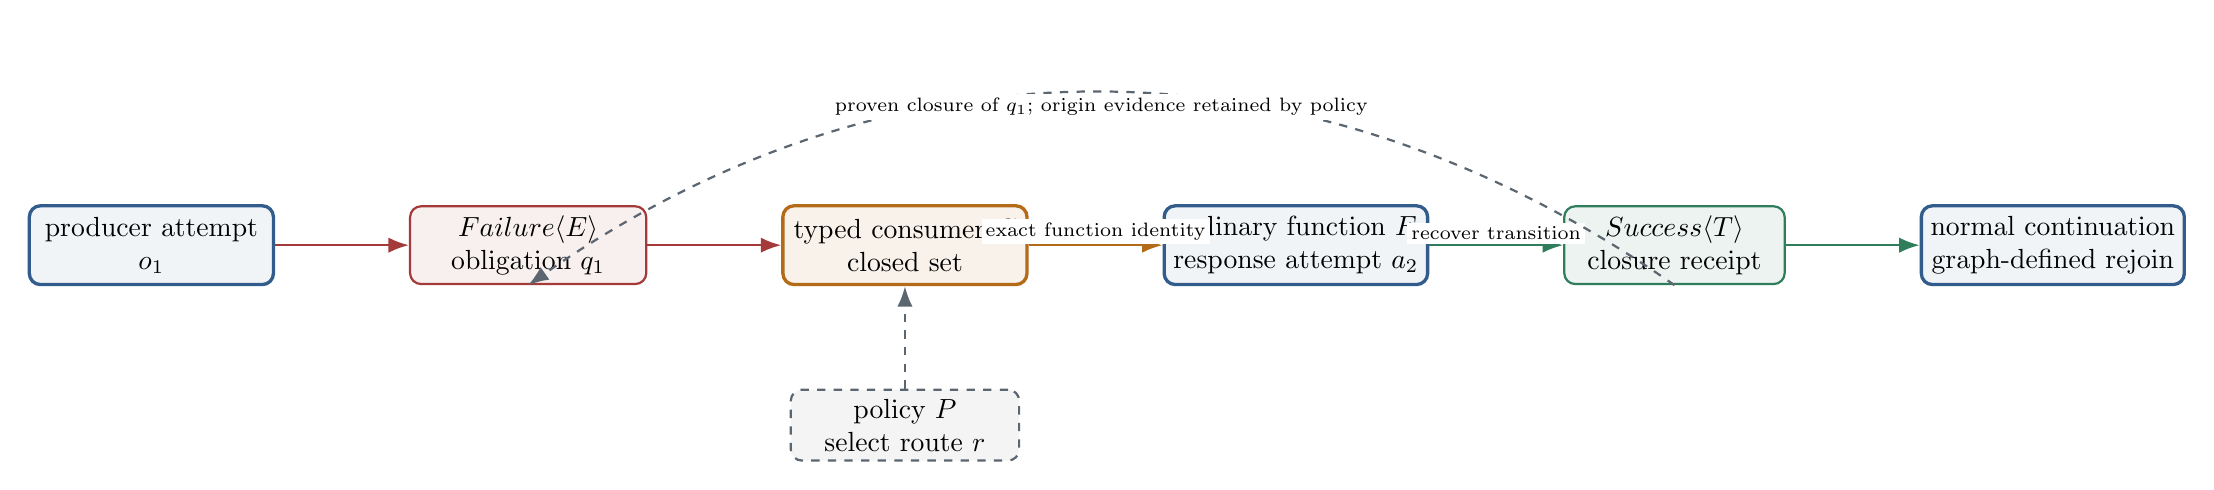
\begin{tikzpicture}[node distance=13mm and 17mm]
  \node[operation] (producer) {producer attempt\\$o_1$};
  \node[failure, right=of producer] (failure) {$Failure\langle E\rangle$\\obligation $q_1$};
  \node[consumer, right=of failure] (consumer) {typed consumer $C$\\closed set};
  \node[policy, below=of consumer] (policy) {policy $P$\\select route $r$};
  \node[operation, right=of consumer] (response) {ordinary function $F$\\response attempt $a_2$};
  \node[success, right=of response] (success) {$Success\langle T\rangle$\\closure receipt};
  \node[operation, right=of success] (continue) {normal continuation\\graph-defined rejoin};
  \draw[failurewire] (producer) -- (failure);
  \draw[failurewire] (failure) -- (consumer);
  \draw[policywire] (policy) -- (consumer);
  \draw[wire, draw=LyraAmber] (consumer) -- node[labelbox, above]{exact function identity} (response);
  \draw[successwire] (response) -- node[labelbox, above]{recover transition} (success);
  \draw[successwire] (success) -- (continue);
  \draw[wire, dashed, bend right=35, draw=LyraGray] (success.south) to
    node[labelbox, below]{proven closure of $q_1$; origin evidence retained by policy} (failure.south);
\end{tikzpicture}}
\end{center}

\section{Decisions required before source or graph admission}

The semantic core is now sufficiently stable to discuss projection choices.
The next review should decide these questions in order:

\begin{enumerate}[leftmargin=*]
  \item \textbf{Producer disposition declaration.} How does a function,
        provider, guard, or operation expose its closed failure and fault set?
  \item \textbf{Envelope parameter spelling.} Is the canonical envelope shown
        as a source type, inferred through a consumer scope, or exposed through
        another explicit projection? Generic type syntax must not be assumed.
  \item \textbf{Consumer declaration shape.} How does source group a closed
        failure set and exact ordinary response functions without dynamic
        nearest-handler lookup or hidden captures?
  \item \textbf{Response-transition spelling.} How is \code{recover T} or
        \code{transform E2} attached to the exact function identity without
        inferring meaning from the body or name?
  \item \textbf{Producer-to-consumer association.} At which explicit source or
        contract boundary is a produced failure wire connected to a consumer?
  \item \textbf{Graph rejoin.} Where may recovered success continue, and which
        identity proves that the normal continuation accepts $T$?
  \item \textbf{Policy location.} Which selections belong in source and which
        remain external versioned policy artifacts?
  \item \textbf{Fault containment.} Define containment separately before any
        fault port can be executable.
\end{enumerate}

Propagation, retry, top-level sinks, cancellation, timeout, backpressure,
multi-failure composition, and evidence storage are deliberately excluded from
this first map. They should be added only after their own semantic contracts
exist.

\section{Recommended review sequence}

\begin{center}
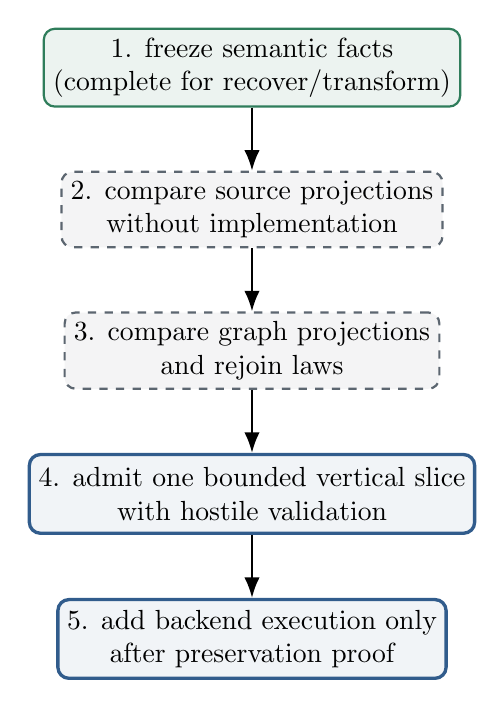
\begin{tikzpicture}[node distance=8mm]
  \node[success] (sem) {1. freeze semantic facts\\(complete for recover/transform)};
  \node[policy, below=of sem] (syntax) {2. compare source projections\\without implementation};
  \node[policy, below=of syntax] (graph) {3. compare graph projections\\and rejoin laws};
  \node[operation, below=of graph] (slice) {4. admit one bounded vertical slice\\with hostile validation};
  \node[operation, below=of slice] (exec) {5. add backend execution only\\after preservation proof};
  \draw[wire] (sem) -- (syntax);
  \draw[wire] (syntax) -- (graph);
  \draw[wire] (graph) -- (slice);
  \draw[wire] (slice) -- (exec);
\end{tikzpicture}
\end{center}

\section*{Authority references}

This map is derived from ADRs 0054--0059, ADR 0062, ADR 0063, the accepted
failure-response disposition decision, Mission 02, and the Gate 2 response
transition checkpoint. The C++ shared contracts remain the mechanically tested
authority for the currently implemented declarative slice.

\end{document}
